\documentclass[10pt,a4paper]{article}
\usepackage[margin=2.1cm]{geometry}
\usepackage[T1]{fontenc}
\usepackage{lmodern,amsmath,graphicx,booktabs,array,longtable,needspace}
\usepackage{url}
\usepackage{hyperref}
\hypersetup{hidelinks,pdftitle={Supporting Information for Coordination Constraints and Information Content in Predicting Lewis Acidity},pdfauthor={Simin Huang, Shenqi Zong, Han Chen, Shaoguang Zhang}}

\setlength{\parindent}{0pt}
\setlength{\parskip}{5pt}
\emergencystretch=2em
\renewcommand{\thefigure}{S\arabic{figure}}
\renewcommand{\thepage}{S\arabic{page}}
\begin{document}
\begin{center}
{\LARGE Supporting Information}\\[8pt]
{\large Coordination Constraints and Information Content in Predicting Lewis Acidity}\\[6pt]
Simin Huang, Shenqi Zong, Han Chen, and Shaoguang Zhang\textsuperscript{*}\\
Tsinghua University, Beijing 100084, China\\
{\small \textsuperscript{*}Department of Chemistry. Email: \href{mailto:sgzhang@tsinghua.edu.cn}{sgzhang@tsinghua.edu.cn}}
\end{center}
\Needspace{9\baselineskip}\section*{S1. Versioned data and complete geometry preparation}

{\footnotesize\setlength{\tabcolsep}{3pt}
\begin{longtable}{@{}>{\raggedright\arraybackslash}p{0.300\textwidth}>{\raggedright\arraybackslash}p{0.190\textwidth}>{\raggedright\arraybackslash}p{0.450\textwidth}@{}}
\toprule
File & Figshare file ID & Verified MD5 \\ \midrule
\endfirsthead
\toprule
File & Figshare file ID & Verified MD5 \\ \midrule
\endhead
FIA49k.csv.gz & 43289211 & 76b9018afda2f8b9c776d1555f55180f \\
FIA49k\_\allowbreak{}predictions.csv.gz & 43289322 & 7f0f55c3e876d34452abd7bbb0c0e657 \\
FIA49k.zip & 43289292 & 60e9ffd7280bdfd6baeb37d6a641f81b \\
\bottomrule
\end{longtable}
}

All 48,986 molecules and 1,617,147 atoms are retained; maximum atom count 118. Atomic numbers: 1, 5, 6, 7, 8, 9, 13, 14, 15, 16, 17, 31, 32, 33, 35, 49, 50, 51, 52, 53, 82, 83. SHA256 fingerprints for the source archives and prepared NPZ are in reports/geometry\_\allowbreak{}provenance.json.

{\footnotesize\setlength{\tabcolsep}{3pt}
\begin{longtable}{@{}>{\raggedright\arraybackslash}p{0.380\textwidth}>{\raggedright\arraybackslash}p{0.570\textwidth}@{}}
\toprule
Assignment & n \\ \midrule
\endfirsthead
\toprule
Assignment & n \\ \midrule
\endhead
train & 32333 \\
validate & 7001 \\
test & 6732 \\
test\_\allowbreak{}2 & 1200 \\
test\_\allowbreak{}4 & 911 \\
test\_\allowbreak{}3 & 763 \\
test\_\allowbreak{}6 & 31 \\
test\_\allowbreak{}5 & 15 \\
\bottomrule
\end{longtable}
}

All atom and target arrays are finite, coordinate row counts are exact, unknown atomic symbols raise an error, and Compound identifiers are unique. No fallback from acid to fluoride-adduct geometry is allowed. The first-atom accepting-center convention is checked against central-element identity for every record. Element-sequence agreement cannot alone exclude permutations of chemically equivalent atoms.

\Needspace{9\baselineskip}\section*{S2. Partition definitions and regression checks}

Generic ligand-scaffold multiset: 12,448 groups containing 46,066 molecules, assigned as 33,460 training, 6,379 validation and 6,227 test records. Individual-ligand overlap with training is 80.8\% in validation and 84.6\% in test.

Exact complete ligand set: 43,226 groups containing 46,066 molecules, assigned as 32,184 training, 6,899 validation and 6,983 test records. Individual-ligand overlap with training is 81.1\% in validation and 80.3\% in test.

Canonical acid identity checking found zero records crossing partitions under the defined RDKit canonicalization. The full canonical grouping keys and molecule identities are included in the machine-readable manifests. Generic scaffold keys retain the multiset of ligand scaffolds; an individual scaffold may recur in a different multiset. Related ligand families and other chemical relationships can consequently span these partitions.

Regression checks cover reproducible disjoint splits, prediction identities and targets, strict geometry parsing, geometric invariance, independent batching, exact checkpoint restoration, training-derived preprocessing, source fingerprints and deterministic ligand grouping. The validation record accompanies the code.

\Needspace{9\baselineskip}\section*{S3. Neural configurations and seed-level test results}

{\footnotesize\setlength{\tabcolsep}{3pt}
\begin{longtable}{@{}>{\raggedright\arraybackslash}p{0.250\textwidth}>{\raggedright\arraybackslash}p{0.096\textwidth}>{\raggedright\arraybackslash}p{0.096\textwidth}>{\raggedright\arraybackslash}p{0.096\textwidth}>{\raggedright\arraybackslash}p{0.096\textwidth}>{\raggedright\arraybackslash}p{0.096\textwidth}>{\raggedright\arraybackslash}p{0.096\textwidth}@{}}
\toprule
Run & Parameters & Epochs & Selected & Val MAE & Test MAE & Test RMSE \\ \midrule
\endfirsthead
\toprule
Run & Parameters & Epochs & Selected & Val MAE & Test MAE & Test RMSE \\ \midrule
\endhead
radial-site-s1 & 378,757 & 86 & 61 & 11.918 & 12.417 & 18.670 \\
radial-site-s2 & 378,757 & 85 & 60 & 11.919 & 12.095 & 18.111 \\
radial-site-s3 & 378,757 & 100 & 97 & 11.844 & 12.161 & 18.491 \\
radial-sum-s1 & 345,989 & 99 & 74 & 11.971 & 12.299 & 18.291 \\
radial-sum-s2 & 345,989 & 87 & 62 & 11.846 & 12.507 & 18.598 \\
radial-sum-s3 & 345,989 & 83 & 58 & 11.873 & 12.373 & 18.716 \\
egnn-sum-s1 & 758,408 & 100 & 83 & 11.944 & 12.255 & 18.883 \\
egnn-sum-s2 & 758,408 & 100 & 99 & 11.699 & 12.013 & 18.285 \\
egnn-sum-s3 & 758,408 & 87 & 62 & 11.720 & 11.965 & 18.524 \\
dimenet-s1 & 1,885,830 & 100 & 94 & 10.496 & 10.993 & 17.010 \\
dimenet-s2 & 1,885,830 & 100 & 83 & 10.834 & 11.506 & 17.732 \\
dimenet-s3 & 1,885,830 & 100 & 99 & 10.583 & 11.119 & 17.276 \\
acid-qm-s1 & 413,061 & 100 & 94 & 11.549 & 12.152 & 18.554 \\
acid-qm-s2 & 413,061 & 93 & 68 & 11.769 & 12.168 & 18.437 \\
acid-qm-s3 & 413,061 & 72 & 47 & 11.759 & 12.222 & 18.804 \\
scaffold-site-s1 & 378,757 & 92 & 67 & 12.558 & 12.630 & 17.886 \\
scaffold-site-s2 & 378,757 & 100 & 98 & 12.407 & 12.790 & 18.182 \\
scaffold-site-s3 & 378,757 & 97 & 72 & 12.520 & 12.893 & 18.380 \\
scaffold-qm-s1 & 413,061 & 53 & 28 & 12.322 & 12.762 & 18.155 \\
scaffold-qm-s2 & 413,061 & 69 & 44 & 12.086 & 12.780 & 18.391 \\
scaffold-qm-s3 & 413,061 & 72 & 47 & 12.213 & 12.713 & 18.180 \\
composition-s1 & 378,757 & 56 & 31 & 28.397 & 28.695 & 39.451 \\
composition-qm-s1 & 413,061 & 64 & 39 & 19.732 & 20.155 & 29.017 \\
\bottomrule
\end{longtable}
}

Scaffold runs report their respective scaffold test. All errors are kJ/mol. Ensemble and seed-average MAEs are reported separately. Runtime records describe observed shared-host epoch wall time. CUDA index\_\allowbreak{}add may produce nondeterministic rounding with fixed RNG seeds. Full configurations, data fingerprints and history logs accompany each checkpoint.

\Needspace{9\baselineskip}\section*{S4. Neural ensemble errors across partitions}

{\footnotesize\setlength{\tabcolsep}{3pt}
\begin{longtable}{@{}>{\raggedright\arraybackslash}p{0.250\textwidth}>{\raggedright\arraybackslash}p{0.120\textwidth}>{\raggedright\arraybackslash}p{0.120\textwidth}>{\raggedright\arraybackslash}p{0.120\textwidth}>{\raggedright\arraybackslash}p{0.120\textwidth}>{\raggedright\arraybackslash}p{0.120\textwidth}@{}}
\toprule
Model & Split & n & MAE & RMSE & R2 \\ \midrule
\endfirsthead
\toprule
Model & Split & n & MAE & RMSE & R2 \\ \midrule
\endhead
radial-site & test & 6732 & 11.152 & 17.225 & 0.9481 \\
radial-site & test\_\allowbreak{}2 & 1200 & 13.398 & 18.432 & 0.9215 \\
radial-site & test\_\allowbreak{}3 & 763 & 23.104 & 30.382 & 0.8720 \\
radial-site & test\_\allowbreak{}4 & 911 & 14.454 & 18.618 & 0.9224 \\
radial-site & test\_\allowbreak{}5 & 15 & 7.615 & 9.583 & 0.8962 \\
radial-site & test\_\allowbreak{}6 & 31 & 10.389 & 14.811 & 0.9322 \\
radial-sum & test & 6732 & 11.222 & 17.222 & 0.9481 \\
radial-sum & test\_\allowbreak{}2 & 1200 & 13.942 & 19.534 & 0.9118 \\
radial-sum & test\_\allowbreak{}3 & 763 & 22.876 & 30.245 & 0.8732 \\
radial-sum & test\_\allowbreak{}4 & 911 & 14.143 & 17.939 & 0.9279 \\
radial-sum & test\_\allowbreak{}5 & 15 & 9.017 & 11.378 & 0.8537 \\
radial-sum & test\_\allowbreak{}6 & 31 & 9.364 & 13.233 & 0.9459 \\
egnn-sum & test & 6732 & 11.044 & 17.298 & 0.9477 \\
egnn-sum & test\_\allowbreak{}2 & 1200 & 13.697 & 19.445 & 0.9126 \\
egnn-sum & test\_\allowbreak{}3 & 763 & 23.544 & 31.357 & 0.8637 \\
egnn-sum & test\_\allowbreak{}4 & 911 & 13.438 & 17.616 & 0.9305 \\
egnn-sum & test\_\allowbreak{}5 & 15 & 3.260 & 5.018 & 0.9715 \\
egnn-sum & test\_\allowbreak{}6 & 31 & 9.018 & 12.131 & 0.9545 \\
dimenet & test & 6732 & 10.288 & 16.394 & 0.9530 \\
dimenet & test\_\allowbreak{}2 & 1200 & 11.931 & 16.809 & 0.9347 \\
dimenet & test\_\allowbreak{}3 & 763 & 20.760 & 27.895 & 0.8921 \\
dimenet & test\_\allowbreak{}4 & 911 & 14.726 & 19.261 & 0.9169 \\
dimenet & test\_\allowbreak{}5 & 15 & 6.392 & 7.609 & 0.9346 \\
dimenet & test\_\allowbreak{}6 & 31 & 4.394 & 6.008 & 0.9888 \\
acid-qm & test & 6732 & 11.125 & 17.423 & 0.9469 \\
acid-qm & test\_\allowbreak{}2 & 1200 & 13.478 & 18.347 & 0.9222 \\
acid-qm & test\_\allowbreak{}3 & 763 & 19.887 & 26.055 & 0.9059 \\
acid-qm & test\_\allowbreak{}4 & 911 & 13.877 & 18.294 & 0.9250 \\
acid-qm & test\_\allowbreak{}5 & 15 & 6.067 & 8.828 & 0.9119 \\
acid-qm & test\_\allowbreak{}6 & 31 & 10.836 & 16.921 & 0.9116 \\
scaffold-site & test & 6227 & 11.660 & 16.828 & 0.9446 \\
scaffold-qm & test & 6227 & 11.705 & 17.009 & 0.9434 \\
composition & test & 6732 & 28.695 & 39.451 & 0.7277 \\
composition & test\_\allowbreak{}2 & 1200 & 37.944 & 48.967 & 0.4457 \\
composition & test\_\allowbreak{}3 & 763 & 33.981 & 43.911 & 0.7326 \\
composition & test\_\allowbreak{}4 & 911 & 25.621 & 33.465 & 0.7492 \\
composition & test\_\allowbreak{}5 & 15 & 36.785 & 40.195 & -0.8258 \\
composition & test\_\allowbreak{}6 & 31 & 25.230 & 33.265 & 0.6582 \\
composition-qm & test & 6732 & 20.155 & 29.017 & 0.8527 \\
composition-qm & test\_\allowbreak{}2 & 1200 & 25.481 & 34.479 & 0.7252 \\
composition-qm & test\_\allowbreak{}3 & 763 & 22.842 & 30.332 & 0.8724 \\
composition-qm & test\_\allowbreak{}4 & 911 & 21.049 & 29.001 & 0.8116 \\
composition-qm & test\_\allowbreak{}5 & 15 & 18.522 & 20.596 & 0.5206 \\
composition-qm & test\_\allowbreak{}6 & 31 & 21.827 & 33.458 & 0.6542 \\
\bottomrule
\end{longtable}
}

\Needspace{9\baselineskip}\section*{S5. Classical baselines and quantum-refinement controls}

qm\_\allowbreak{}baseline

{\footnotesize\setlength{\tabcolsep}{3pt}
\begin{longtable}{@{}>{\raggedright\arraybackslash}p{0.310\textwidth}>{\raggedright\arraybackslash}p{0.141\textwidth}>{\raggedright\arraybackslash}p{0.141\textwidth}>{\raggedright\arraybackslash}p{0.141\textwidth}>{\raggedright\arraybackslash}p{0.141\textwidth}@{}}
\toprule
Model & Split & n & MAE & RMSE \\ \midrule
\endfirsthead
\toprule
Model & Split & n & MAE & RMSE \\ \midrule
\endhead
metadata & test & 6732 & 37.569 & 49.465 \\
metadata & test\_\allowbreak{}2 & 1200 & 51.748 & 62.948 \\
metadata & test\_\allowbreak{}3 & 763 & 54.034 & 63.876 \\
metadata & test\_\allowbreak{}4 & 911 & 39.702 & 48.455 \\
metadata & test\_\allowbreak{}5 & 15 & 42.694 & 47.346 \\
metadata & test\_\allowbreak{}6 & 31 & 81.991 & 92.345 \\
metadata\_\allowbreak{}plus\_\allowbreak{}LA\_\allowbreak{}QM & test & 6732 & 23.020 & 31.939 \\
metadata\_\allowbreak{}plus\_\allowbreak{}LA\_\allowbreak{}QM & test\_\allowbreak{}2 & 1200 & 29.262 & 38.617 \\
metadata\_\allowbreak{}plus\_\allowbreak{}LA\_\allowbreak{}QM & test\_\allowbreak{}3 & 763 & 25.799 & 33.267 \\
metadata\_\allowbreak{}plus\_\allowbreak{}LA\_\allowbreak{}QM & test\_\allowbreak{}4 & 911 & 21.361 & 28.366 \\
metadata\_\allowbreak{}plus\_\allowbreak{}LA\_\allowbreak{}QM & test\_\allowbreak{}5 & 15 & 39.281 & 40.008 \\
metadata\_\allowbreak{}plus\_\allowbreak{}LA\_\allowbreak{}QM & test\_\allowbreak{}6 & 31 & 39.802 & 59.367 \\
\bottomrule
\end{longtable}
}

rdkit\_\allowbreak{}baseline

{\footnotesize\setlength{\tabcolsep}{3pt}
\begin{longtable}{@{}>{\raggedright\arraybackslash}p{0.310\textwidth}>{\raggedright\arraybackslash}p{0.141\textwidth}>{\raggedright\arraybackslash}p{0.141\textwidth}>{\raggedright\arraybackslash}p{0.141\textwidth}>{\raggedright\arraybackslash}p{0.141\textwidth}@{}}
\toprule
Model & Split & n & MAE & RMSE \\ \midrule
\endfirsthead
\toprule
Model & Split & n & MAE & RMSE \\ \midrule
\endhead
RDKit2D & test & 6732 & 18.729 & 25.821 \\
RDKit2D & test\_\allowbreak{}2 & 1200 & 23.198 & 30.162 \\
RDKit2D & test\_\allowbreak{}3 & 763 & 24.989 & 33.197 \\
RDKit2D & test\_\allowbreak{}4 & 911 & 21.162 & 28.056 \\
RDKit2D & test\_\allowbreak{}5 & 15 & 27.060 & 31.027 \\
RDKit2D & test\_\allowbreak{}6 & 31 & 9.288 & 12.577 \\
RDKit2D\_\allowbreak{}plus\_\allowbreak{}LA\_\allowbreak{}QM & test & 6732 & 17.347 & 24.176 \\
RDKit2D\_\allowbreak{}plus\_\allowbreak{}LA\_\allowbreak{}QM & test\_\allowbreak{}2 & 1200 & 22.978 & 29.944 \\
RDKit2D\_\allowbreak{}plus\_\allowbreak{}LA\_\allowbreak{}QM & test\_\allowbreak{}3 & 763 & 21.848 & 29.331 \\
RDKit2D\_\allowbreak{}plus\_\allowbreak{}LA\_\allowbreak{}QM & test\_\allowbreak{}4 & 911 & 18.034 & 24.415 \\
RDKit2D\_\allowbreak{}plus\_\allowbreak{}LA\_\allowbreak{}QM & test\_\allowbreak{}5 & 15 & 25.807 & 28.398 \\
RDKit2D\_\allowbreak{}plus\_\allowbreak{}LA\_\allowbreak{}QM & test\_\allowbreak{}6 & 31 & 21.501 & 30.282 \\
\bottomrule
\end{longtable}
}

refinement

{\footnotesize\setlength{\tabcolsep}{3pt}
\begin{longtable}{@{}>{\raggedright\arraybackslash}p{0.310\textwidth}>{\raggedright\arraybackslash}p{0.141\textwidth}>{\raggedright\arraybackslash}p{0.141\textwidth}>{\raggedright\arraybackslash}p{0.141\textwidth}>{\raggedright\arraybackslash}p{0.141\textwidth}@{}}
\toprule
Model & Split & n & MAE & RMSE \\ \midrule
\endfirsthead
\toprule
Model & Split & n & MAE & RMSE \\ \midrule
\endhead
PBEh3c\_\allowbreak{}raw & test & 6732 & 23.332 & 26.268 \\
PBEh3c\_\allowbreak{}raw & test\_\allowbreak{}2 & 1200 & 26.732 & 29.532 \\
PBEh3c\_\allowbreak{}raw & test\_\allowbreak{}3 & 763 & 29.759 & 32.182 \\
PBEh3c\_\allowbreak{}raw & test\_\allowbreak{}4 & 911 & 26.639 & 29.333 \\
PBEh3c\_\allowbreak{}raw & test\_\allowbreak{}5 & 15 & 14.195 & 15.127 \\
PBEh3c\_\allowbreak{}raw & test\_\allowbreak{}6 & 31 & 14.635 & 16.728 \\
PBEh3c\_\allowbreak{}global\_\allowbreak{}bias & test & 6732 & 10.062 & 12.616 \\
PBEh3c\_\allowbreak{}global\_\allowbreak{}bias & test\_\allowbreak{}2 & 1200 & 10.674 & 13.322 \\
PBEh3c\_\allowbreak{}global\_\allowbreak{}bias & test\_\allowbreak{}3 & 763 & 11.307 & 14.129 \\
PBEh3c\_\allowbreak{}global\_\allowbreak{}bias & test\_\allowbreak{}4 & 911 & 9.999 & 12.945 \\
PBEh3c\_\allowbreak{}global\_\allowbreak{}bias & test\_\allowbreak{}5 & 15 & 9.783 & 10.195 \\
PBEh3c\_\allowbreak{}global\_\allowbreak{}bias & test\_\allowbreak{}6 & 31 & 9.739 & 11.753 \\
PBEh3c\_\allowbreak{}class\_\allowbreak{}bias & test & 6732 & 7.149 & 9.218 \\
PBEh3c\_\allowbreak{}class\_\allowbreak{}bias & test\_\allowbreak{}2 & 1200 & 8.407 & 10.854 \\
PBEh3c\_\allowbreak{}class\_\allowbreak{}bias & test\_\allowbreak{}3 & 763 & 8.332 & 10.328 \\
PBEh3c\_\allowbreak{}class\_\allowbreak{}bias & test\_\allowbreak{}4 & 911 & 6.821 & 8.748 \\
PBEh3c\_\allowbreak{}class\_\allowbreak{}bias & test\_\allowbreak{}5 & 15 & 3.231 & 5.589 \\
PBEh3c\_\allowbreak{}class\_\allowbreak{}bias & test\_\allowbreak{}6 & 31 & 6.818 & 8.613 \\
delta\_\allowbreak{}metadata & test & 6732 & 4.845 & 6.314 \\
delta\_\allowbreak{}metadata & test\_\allowbreak{}2 & 1200 & 6.938 & 8.734 \\
delta\_\allowbreak{}metadata & test\_\allowbreak{}3 & 763 & 5.000 & 6.492 \\
delta\_\allowbreak{}metadata & test\_\allowbreak{}4 & 911 & 3.789 & 5.026 \\
delta\_\allowbreak{}metadata & test\_\allowbreak{}5 & 15 & 5.371 & 6.428 \\
delta\_\allowbreak{}metadata & test\_\allowbreak{}6 & 31 & 3.208 & 4.080 \\
delta\_\allowbreak{}RDKit\_\allowbreak{}LA\_\allowbreak{}QM & test & 6732 & 3.289 & 4.485 \\
delta\_\allowbreak{}RDKit\_\allowbreak{}LA\_\allowbreak{}QM & test\_\allowbreak{}2 & 1200 & 3.765 & 4.897 \\
delta\_\allowbreak{}RDKit\_\allowbreak{}LA\_\allowbreak{}QM & test\_\allowbreak{}3 & 763 & 4.034 & 5.193 \\
delta\_\allowbreak{}RDKit\_\allowbreak{}LA\_\allowbreak{}QM & test\_\allowbreak{}4 & 911 & 3.030 & 4.092 \\
delta\_\allowbreak{}RDKit\_\allowbreak{}LA\_\allowbreak{}QM & test\_\allowbreak{}5 & 15 & 4.298 & 4.773 \\
delta\_\allowbreak{}RDKit\_\allowbreak{}LA\_\allowbreak{}QM & test\_\allowbreak{}6 & 31 & 2.323 & 2.832 \\
\bottomrule
\end{longtable}
}

grouped\_\allowbreak{}scaffold

{\footnotesize\setlength{\tabcolsep}{3pt}
\begin{longtable}{@{}>{\raggedright\arraybackslash}p{0.310\textwidth}>{\raggedright\arraybackslash}p{0.141\textwidth}>{\raggedright\arraybackslash}p{0.141\textwidth}>{\raggedright\arraybackslash}p{0.141\textwidth}>{\raggedright\arraybackslash}p{0.141\textwidth}@{}}
\toprule
Model & Split & n & MAE & RMSE \\ \midrule
\endfirsthead
\toprule
Model & Split & n & MAE & RMSE \\ \midrule
\endhead
RDKit2D & test & 6227 & 19.095 & 26.180 \\
delta\_\allowbreak{}RDKit\_\allowbreak{}LA\_\allowbreak{}QM & test & 6227 & 3.348 & 4.453 \\
\bottomrule
\end{longtable}
}

The final HGB stage budget is matched across primary, grouped and refinement experiments: stages 100/400/1000 are selected on validation only. Every fitted feature list and selection score is saved in the corresponding config.json. The lower-level FIA in refinement is an explicit adduct-dependent input; it is not included in the acid-QM fusion models.

\Needspace{9\baselineskip}\section*{S6. Paired uncertainty and subgroup interpretation}

{\footnotesize\setlength{\tabcolsep}{3pt}
\begin{longtable}{@{}>{\raggedright\arraybackslash}p{0.310\textwidth}>{\raggedright\arraybackslash}p{0.141\textwidth}>{\raggedright\arraybackslash}p{0.141\textwidth}>{\raggedright\arraybackslash}p{0.141\textwidth}>{\raggedright\arraybackslash}p{0.141\textwidth}@{}}
\toprule
Model & Split & $\Delta$ MAE & 95\% lower & 95\% upper \\ \midrule
\endfirsthead
\toprule
Model & Split & $\Delta$ MAE & 95\% lower & 95\% upper \\ \midrule
\endhead
radial-site & test & -0.960 & -1.194 & -0.729 \\
radial-site & test\_\allowbreak{}2 & -1.041 & -1.731 & -0.365 \\
radial-site & test\_\allowbreak{}3 & -0.977 & -2.054 & 0.116 \\
radial-site & test\_\allowbreak{}4 & -3.480 & -4.289 & -2.663 \\
radial-site & test\_\allowbreak{}5 & -3.308 & -7.129 & 1.392 \\
radial-site & test\_\allowbreak{}6 & 1.858 & 0.886 & 2.855 \\
radial-sum & test & -0.890 & -1.121 & -0.658 \\
radial-sum & test\_\allowbreak{}2 & -0.498 & -1.204 & 0.238 \\
radial-sum & test\_\allowbreak{}3 & -1.204 & -2.321 & -0.087 \\
radial-sum & test\_\allowbreak{}4 & -3.791 & -4.625 & -2.988 \\
radial-sum & test\_\allowbreak{}5 & -1.905 & -5.902 & 3.183 \\
radial-sum & test\_\allowbreak{}6 & 0.834 & -0.379 & 2.031 \\
egnn-sum & test & -1.068 & -1.313 & -0.837 \\
egnn-sum & test\_\allowbreak{}2 & -0.742 & -1.422 & -0.043 \\
egnn-sum & test\_\allowbreak{}3 & -0.537 & -1.718 & 0.590 \\
egnn-sum & test\_\allowbreak{}4 & -4.496 & -5.174 & -3.811 \\
egnn-sum & test\_\allowbreak{}5 & -7.662 & -10.714 & -4.395 \\
egnn-sum & test\_\allowbreak{}6 & 0.487 & -0.808 & 1.733 \\
dimenet & test & -1.824 & -2.060 & -1.592 \\
dimenet & test\_\allowbreak{}2 & -2.509 & -3.196 & -1.808 \\
dimenet & test\_\allowbreak{}3 & -3.321 & -4.509 & -2.179 \\
dimenet & test\_\allowbreak{}4 & -3.208 & -4.241 & -2.252 \\
dimenet & test\_\allowbreak{}5 & -4.531 & -7.537 & -1.209 \\
dimenet & test\_\allowbreak{}6 & -4.136 & -4.971 & -3.299 \\
acid-qm & test & -0.987 & -1.227 & -0.749 \\
acid-qm & test\_\allowbreak{}2 & -0.962 & -1.661 & -0.258 \\
acid-qm & test\_\allowbreak{}3 & -4.193 & -5.474 & -2.938 \\
acid-qm & test\_\allowbreak{}4 & -4.057 & -4.981 & -3.163 \\
acid-qm & test\_\allowbreak{}5 & -4.856 & -8.492 & -0.166 \\
acid-qm & test\_\allowbreak{}6 & 2.305 & 0.978 & 3.573 \\
scaffold-site & test & -7.435 & -7.809 & -7.049 \\
scaffold-qm & test & -7.390 & -7.770 & -7.000 \\
composition & test & 16.583 & 15.952 & 17.190 \\
composition & test\_\allowbreak{}2 & 23.504 & 21.795 & 25.210 \\
composition & test\_\allowbreak{}3 & 9.900 & 8.089 & 11.715 \\
composition & test\_\allowbreak{}4 & 7.687 & 6.420 & 8.983 \\
composition & test\_\allowbreak{}5 & 25.862 & 17.058 & 34.221 \\
composition & test\_\allowbreak{}6 & 16.699 & 14.655 & 18.698 \\
composition-qm & test & 8.043 & 7.611 & 8.483 \\
composition-qm & test\_\allowbreak{}2 & 11.041 & 9.794 & 12.399 \\
composition-qm & test\_\allowbreak{}3 & -1.239 & -2.840 & 0.355 \\
composition-qm & test\_\allowbreak{}4 & 3.115 & 2.087 & 4.131 \\
composition-qm & test\_\allowbreak{}5 & 7.599 & 3.193 & 12.941 \\
composition-qm & test\_\allowbreak{}6 & 13.297 & 11.173 & 15.557 \\
\bottomrule
\end{longtable}
}

$\Delta$ MAE is new-model ensemble error minus reference error; negative values favor the new model. Official-partition reference: released FIA-GNN. Scaffold reference: the independently refitted RDKit HGB baseline. Each bootstrap resample preserves central-class counts and pairs predictions on the same molecules. These intervals condition on the fitted weights. The complete by\_\allowbreak{}class.csv contains per-class n, target variance, MAE, RMSE and R2; small classes and low-variance targets require caution.

\Needspace{9\baselineskip}\section*{S7. Geometry-source and paired-structure diagnostics}

{\footnotesize\setlength{\tabcolsep}{3pt}
\begin{longtable}{@{}>{\raggedright\arraybackslash}p{0.250\textwidth}>{\raggedright\arraybackslash}p{0.120\textwidth}>{\raggedright\arraybackslash}p{0.120\textwidth}>{\raggedright\arraybackslash}p{0.120\textwidth}>{\raggedright\arraybackslash}p{0.120\textwidth}>{\raggedright\arraybackslash}p{0.120\textwidth}@{}}
\toprule
Seed & Split & xTB MAE & PBEh MAE & $\Delta$ MAE & Mean |$\Delta$ prediction| \\ \midrule
\endfirsthead
\toprule
Seed & Split & xTB MAE & PBEh MAE & $\Delta$ MAE & Mean |$\Delta$ prediction| \\ \midrule
\endhead
1 & test & 14.385 & 12.417 & 1.969 & 7.117 \\
1 & test\_\allowbreak{}2 & 16.621 & 14.913 & 1.709 & 6.848 \\
1 & test\_\allowbreak{}3 & 26.005 & 24.738 & 1.267 & 7.876 \\
1 & test\_\allowbreak{}4 & 16.647 & 15.921 & 0.726 & 5.127 \\
1 & test\_\allowbreak{}5 & 11.279 & 8.116 & 3.162 & 3.903 \\
1 & test\_\allowbreak{}6 & 16.706 & 13.330 & 3.376 & 5.282 \\
2 & test & 13.919 & 12.095 & 1.824 & 7.196 \\
2 & test\_\allowbreak{}2 & 16.117 & 14.717 & 1.401 & 6.504 \\
2 & test\_\allowbreak{}3 & 25.641 & 23.918 & 1.724 & 7.571 \\
2 & test\_\allowbreak{}4 & 16.239 & 15.527 & 0.712 & 4.959 \\
2 & test\_\allowbreak{}5 & 10.860 & 8.484 & 2.376 & 3.298 \\
2 & test\_\allowbreak{}6 & 10.419 & 7.835 & 2.583 & 5.942 \\
3 & test & 14.022 & 12.161 & 1.860 & 6.992 \\
3 & test\_\allowbreak{}2 & 16.354 & 14.961 & 1.393 & 6.513 \\
3 & test\_\allowbreak{}3 & 26.121 & 24.795 & 1.326 & 7.639 \\
3 & test\_\allowbreak{}4 & 16.070 & 14.907 & 1.163 & 5.560 \\
3 & test\_\allowbreak{}5 & 8.843 & 8.227 & 0.616 & 2.832 \\
3 & test\_\allowbreak{}6 & 17.693 & 12.877 & 4.816 & 7.212 \\
\bottomrule
\end{longtable}
}

Paired acid/adduct structure check: N\_\allowbreak{}adduct=N\_\allowbreak{}acid+1; all preceding Z equal; final Z=9; xTB Z equal. Element-sequence equality checks the archive order convention; identical-element atom permutations cannot be excluded by Z alone.

The heavy-atom pair-distance RMS change is sqrt(mean[(d\_\allowbreak{}ij,adduct - d\_\allowbreak{}ij,acid)\textasciicircum{}2]) over unordered heavy-atom pairs. The 2.7 Å center-shell cutoff is geometric and does not assign covalent bonds. Distances are in Å. The added fluoride is the final atom in the checked archive convention. These released geometries are used for structural diagnostics, independently of any energetic deformation analysis. The full 48,986-row geometry diagnostic export is included in the archive.

\clearpage

\Needspace{9\baselineskip}\section*{S8. Matched-ligand reference-method corrections}

{\footnotesize\setlength{\tabcolsep}{3pt}
\begin{longtable}{@{}>{\raggedright\arraybackslash}p{0.250\textwidth}>{\raggedright\arraybackslash}p{0.120\textwidth}>{\raggedright\arraybackslash}p{0.120\textwidth}>{\raggedright\arraybackslash}p{0.120\textwidth}>{\raggedright\arraybackslash}p{0.120\textwidth}>{\raggedright\arraybackslash}p{0.120\textwidth}@{}}
\toprule
Center A & Center B & Ligand sets & B - A & 95\% lower & 95\% upper \\ \midrule
\endfirsthead
\toprule
Center A & Center B & Ligand sets & B - A & 95\% lower & 95\% upper \\ \midrule
\endhead
P(III) & As(III) & 34 & 2.662 & 0.838 & 4.621 \\
As(III) & Sb(III) & 69 & -0.808 & -2.183 & 0.605 \\
Sb(III) & Bi(III) & 74 & 4.156 & 3.552 & 4.705 \\
Si(IV) & Ge(IV) & 30 & 2.502 & 0.552 & 4.465 \\
Ge(IV) & Sn(IV) & 22 & -1.648 & -3.683 & 0.337 \\
Sn(IV) & Pb(IV) & 10 & 5.413 & 3.202 & 7.480 \\
Si(II) & Ge(II) & 90 & -0.083 & -0.838 & 0.728 \\
Ge(II) & Sn(II) & 98 & 6.400 & 5.763 & 7.033 \\
Sn(II) & Pb(II) & 103 & 6.349 & 6.005 & 6.681 \\
\bottomrule
\end{longtable}
}

The correction is FIA(DSD-BLYP) minus FIA(PBEh-3c), in kJ/mol. Comparisons use only training molecules. Repeated records are averaged within each canonical ligand-set/center-class cell before pairing. The nine neighboring-center contrasts were defined before inspection and are all retained. Intervals use 2,000 bootstrap samples over matched ligand sets with seed 20261113; they are descriptive, without a multiple-testing significance claim.

\Needspace{9\baselineskip}\section*{S9. Reproduction and provenance}

README.md gives the preparation, training, evaluation and analysis commands. reports/experiment\_\allowbreak{}plan.json distinguishes the initial fixed comparisons from exploratory acid-QM and geometry-source extensions. requirements-benchmark.txt and run configurations record the software environment; THIRD\_\allowbreak{}PARTY.md records upstream code commits and licenses. A frozen archive contains split identities, all prediction exports, histories and checkpoints, together with a checksum manifest. The storage manifest provides SHA256 verification for each restored file.

\Needspace{9\baselineskip}\section*{S10. Chemical environments and paired-structure analysis}

Chemical subgroup analyses are exploratory evaluations of frozen models on all 6,732 main-test molecules. Bins use training-set percentiles. The binding-induced heavy-atom pair-distance RMS thresholds are 0.278968, 0.532265, 0.837720, 1.173082 Å. The PBEh-3c/GFN2-xTB geometry-disagreement thresholds are 0.127501, 0.226552, 0.386364 Å. Intervals use 2,000 central-class-stratified molecule bootstrap samples with seed 20261114 and fixed fitted models.

All main-test molecules by ligand denticity

{\footnotesize\setlength{\tabcolsep}{3pt}
\begin{longtable}{@{}>{\raggedright\arraybackslash}p{0.250\textwidth}>{\raggedright\arraybackslash}p{0.120\textwidth}>{\raggedright\arraybackslash}p{0.120\textwidth}>{\raggedright\arraybackslash}p{0.120\textwidth}>{\raggedright\arraybackslash}p{0.120\textwidth}>{\raggedright\arraybackslash}p{0.120\textwidth}@{}}
\toprule
Group & Model / contrast & n & MAE / gain & 95\% lower & 95\% upper \\ \midrule
\endfirsthead
\toprule
Group & Model / contrast & n & MAE / gain & 95\% lower & 95\% upper \\ \midrule
\endhead
bi & FIA-GNN & 2610 & 10.646 & 10.264 & 11.059 \\
bi & DimeNet++ & 2610 & 8.873 & 8.535 & 9.221 \\
bi & Refinement & 2610 & 3.022 & 2.930 & 3.124 \\
bi & 3D gain over FIA-GNN & 2610 & 1.773 & 1.456 & 2.107 \\
mono & FIA-GNN & 2247 & 10.511 & 10.126 & 10.917 \\
mono & DimeNet++ & 2247 & 9.070 & 8.729 & 9.403 \\
mono & Refinement & 2247 & 3.354 & 3.235 & 3.489 \\
mono & 3D gain over FIA-GNN & 2247 & 1.441 & 1.120 & 1.794 \\
tri & FIA-GNN & 1875 & 16.071 & 15.132 & 17.038 \\
tri & DimeNet++ & 1875 & 13.718 & 12.912 & 14.587 \\
tri & Refinement & 1875 & 3.584 & 3.434 & 3.741 \\
tri & 3D gain over FIA-GNN & 1875 & 2.353 & 1.768 & 2.943 \\
\bottomrule
\end{longtable}
}

P(III) by ligand denticity

{\footnotesize\setlength{\tabcolsep}{3pt}
\begin{longtable}{@{}>{\raggedright\arraybackslash}p{0.250\textwidth}>{\raggedright\arraybackslash}p{0.120\textwidth}>{\raggedright\arraybackslash}p{0.120\textwidth}>{\raggedright\arraybackslash}p{0.120\textwidth}>{\raggedright\arraybackslash}p{0.120\textwidth}>{\raggedright\arraybackslash}p{0.120\textwidth}@{}}
\toprule
Group & Model / contrast & n & MAE / gain & 95\% lower & 95\% upper \\ \midrule
\endfirsthead
\toprule
Group & Model / contrast & n & MAE / gain & 95\% lower & 95\% upper \\ \midrule
\endhead
bi & FIA-GNN & 83 & 21.010 & 17.089 & 25.895 \\
bi & DimeNet++ & 83 & 17.978 & 14.447 & 22.138 \\
bi & Refinement & 83 & 3.599 & 2.945 & 4.317 \\
bi & 3D gain over FIA-GNN & 83 & 3.031 & 0.115 & 6.003 \\
mono & FIA-GNN & 59 & 16.356 & 12.476 & 20.562 \\
mono & DimeNet++ & 59 & 18.766 & 15.038 & 22.482 \\
mono & Refinement & 59 & 2.619 & 2.074 & 3.217 \\
mono & 3D gain over FIA-GNN & 59 & -2.410 & -5.820 & 0.750 \\
tri & FIA-GNN & 77 & 20.544 & 15.421 & 26.455 \\
tri & DimeNet++ & 77 & 15.970 & 11.875 & 20.561 \\
tri & Refinement & 77 & 3.890 & 3.197 & 4.622 \\
tri & 3D gain over FIA-GNN & 77 & 4.574 & 0.903 & 8.308 \\
\bottomrule
\end{longtable}
}

P(III) by training-defined angle-sum quartile

{\footnotesize\setlength{\tabcolsep}{3pt}
\begin{longtable}{@{}>{\raggedright\arraybackslash}p{0.250\textwidth}>{\raggedright\arraybackslash}p{0.120\textwidth}>{\raggedright\arraybackslash}p{0.120\textwidth}>{\raggedright\arraybackslash}p{0.120\textwidth}>{\raggedright\arraybackslash}p{0.120\textwidth}>{\raggedright\arraybackslash}p{0.120\textwidth}@{}}
\toprule
Group & Model / contrast & n & MAE / gain & 95\% lower & 95\% upper \\ \midrule
\endfirsthead
\toprule
Group & Model / contrast & n & MAE / gain & 95\% lower & 95\% upper \\ \midrule
\endhead
Q4 & FIA-GNN & 44 & 21.906 & 13.952 & 31.227 \\
Q4 & DimeNet++ & 44 & 20.186 & 14.239 & 26.796 \\
Q4 & Refinement & 44 & 3.129 & 2.397 & 3.913 \\
Q4 & 3D gain over FIA-GNN & 44 & 1.720 & -3.458 & 7.080 \\
Q1 & FIA-GNN & 66 & 21.592 & 16.529 & 27.110 \\
Q1 & DimeNet++ & 66 & 17.945 & 13.746 & 22.957 \\
Q1 & Refinement & 66 & 3.521 & 2.780 & 4.367 \\
Q1 & 3D gain over FIA-GNN & 66 & 3.647 & 0.303 & 6.897 \\
Q2 & FIA-GNN & 66 & 16.690 & 13.312 & 20.444 \\
Q2 & DimeNet++ & 66 & 14.887 & 11.514 & 18.331 \\
Q2 & Refinement & 66 & 3.075 & 2.513 & 3.714 \\
Q2 & 3D gain over FIA-GNN & 66 & 1.802 & -0.966 & 4.527 \\
Q3 & FIA-GNN & 43 & 18.609 & 14.529 & 23.061 \\
Q3 & DimeNet++ & 43 & 17.999 & 13.426 & 23.672 \\
Q3 & Refinement & 43 & 4.182 & 3.206 & 5.257 \\
Q3 & 3D gain over FIA-GNN & 43 & 0.610 & -4.098 & 4.988 \\
\bottomrule
\end{longtable}
}

Gain is FIA-GNN absolute error minus DimeNet++ absolute error on the same molecules. Positive values favor the geometric predictor. Local geometry is represented by the sum of three first-shell interligand angles; P(III) quartile thresholds are 291.6494, 295.6974, 300.1256 degrees. First-shell assignments match the reported element composition with the nearest atoms of each element. Across 19,691 three-coordinate structures, the maximum assigned distance divided by the sum of covalent radii is 1.1924. Assigned atom indices and geometry descriptors are regenerated by lewis\_\allowbreak{}acidity.chemistry\_\allowbreak{}insights.

{\footnotesize\setlength{\tabcolsep}{3pt}
\begin{longtable}{@{}>{\raggedright\arraybackslash}p{0.250\textwidth}>{\raggedright\arraybackslash}p{0.120\textwidth}>{\raggedright\arraybackslash}p{0.120\textwidth}>{\raggedright\arraybackslash}p{0.120\textwidth}>{\raggedright\arraybackslash}p{0.120\textwidth}>{\raggedright\arraybackslash}p{0.120\textwidth}@{}}
\toprule
Center & n & DimeNet++ & EGNN & Acid QM & Refinement \\ \midrule
\endfirsthead
\toprule
Center & n & DimeNet++ & EGNN & Acid QM & Refinement \\ \midrule
\endhead
Al(III) & 325 & 7.183 & 8.022 & 7.828 & 2.672 \\
As(III) & 339 & 12.509 & 11.764 & 13.172 & 3.978 \\
As(V) & 363 & 11.216 & 12.436 & 13.283 & 3.910 \\
B(III) & 428 & 11.984 & 13.102 & 13.356 & 3.051 \\
Bi(III) & 383 & 9.256 & 9.920 & 9.179 & 3.223 \\
Bi(V) & 314 & 10.766 & 11.125 & 11.500 & 4.378 \\
Ga(III) & 331 & 7.761 & 8.464 & 8.867 & 2.629 \\
Ge(II) & 221 & 7.087 & 7.482 & 6.820 & 2.349 \\
Ge(IV) & 400 & 10.392 & 11.184 & 12.020 & 3.377 \\
In(III) & 285 & 7.312 & 8.022 & 7.478 & 2.785 \\
P(III) & 219 & 17.484 & 17.544 & 17.759 & 3.438 \\
P(V) & 323 & 14.079 & 16.312 & 16.127 & 4.684 \\
Pb(II) & 235 & 6.068 & 6.578 & 5.625 & 2.377 \\
Pb(IV) & 244 & 10.489 & 10.532 & 11.128 & 3.461 \\
Sb(III) & 408 & 9.022 & 10.309 & 9.914 & 2.905 \\
Sb(V) & 343 & 10.935 & 11.797 & 12.133 & 3.529 \\
Si(II) & 244 & 7.493 & 7.793 & 7.776 & 2.361 \\
Si(IV) & 393 & 12.865 & 13.213 & 13.787 & 3.497 \\
Sn(II) & 228 & 5.684 & 5.851 & 5.067 & 2.245 \\
Sn(IV) & 321 & 10.479 & 11.947 & 12.187 & 3.587 \\
Te(IV) & 385 & 12.589 & 13.977 & 13.277 & 3.581 \\
\bottomrule
\end{longtable}
}

{\footnotesize\setlength{\tabcolsep}{3pt}
\begin{longtable}{@{}>{\raggedright\arraybackslash}p{0.310\textwidth}>{\raggedright\arraybackslash}p{0.141\textwidth}>{\raggedright\arraybackslash}p{0.141\textwidth}>{\raggedright\arraybackslash}p{0.141\textwidth}>{\raggedright\arraybackslash}p{0.141\textwidth}@{}}
\toprule
Source percentile & n & MAE increase & 95\% lower & 95\% upper \\ \midrule
\endfirsthead
\toprule
Source percentile & n & MAE increase & 95\% lower & 95\% upper \\ \midrule
\endhead
P0--50 & 3378.0 & 1.045 & 0.867 & 1.232 \\
P50--75 & 1623.0 & 1.882 & 1.531 & 2.244 \\
P75--90 & 1028.0 & 2.486 & 1.934 & 3.088 \\
P90--100 & 703.0 & 4.915 & 3.963 & 5.852 \\
\bottomrule
\end{longtable}
}

Giving each of the 21 center classes equal weight yields geometry-source penalties of 1.679 kJ/mol below the training upper-decile threshold and 3.761 kJ/mol above it. Paired-geometry disagreement is evaluated where both protocols are available. The source-change experiment retains PBEh-trained weights; independent xTB-domain training is a separate modeling task.

\Needspace{9\baselineskip}\section*{S11. Relationship to contemporary studies}

{\footnotesize\setlength{\tabcolsep}{3pt}
\begin{longtable}{@{}>{\raggedright\arraybackslash}p{0.160\textwidth}>{\raggedright\arraybackslash}p{0.240\textwidth}>{\raggedright\arraybackslash}p{0.240\textwidth}>{\raggedright\arraybackslash}p{0.280\textwidth}@{}}
\toprule
Study & Endpoint and domain & Molecular information & Contribution and relationship \\ \midrule
\endfirsthead
\toprule
Study & Endpoint and domain & Molecular information & Contribution and relationship \\ \midrule
\endhead
Sigmund et al. \cite{sigmund2024fia} & Gas/solution FIA; 48,986 p-block acids & Connectivity and chemical metadata & FIA49k and broad FIA-GNN prediction. Released predictions provide the same-molecule reference in the present work. \\
Fenogli et al. \cite{fenogli2025boron} & FIA; 594 boron acids in four scaffold families & Quantum, substituent-based and cheminformatics descriptors & Interpretable substituent design rules in focused chemical spaces. The present study evaluates broad p-block coordination classes and ligand-combination transfer. \\
Kirsch et al. \cite{kirsch2025pnictogen} & FIA and electronic/steric properties; 16 pincer frameworks and four pnictogens & Quantum-chemical structures and electronic analysis & Geometry and ligand-dependent pnictogen chemistry. The present analysis examines predictive information across the broader FIA49k population. \\
Mahdian et al. \cite{mahdian2026base} & 3,927 adduct free energies; 816 boranes and five bases & DFT and chemically informed descriptors & Quantifies substituent effects and base-dependent acidity rankings. The present target is gas-phase fluoride-binding enthalpy. \\
Bhattacharya et al. \cite{bhattacharya2026proton} & Gas-phase proton affinities; experimental and DFT references & PM7 binding estimates, electronic and cheminformatics descriptors & Multi-fidelity correction and prospective screening. The present work applies established correction learning to FIA and resolves coordination, central-element and geometry-source dependence. \\
\bottomrule
\end{longtable}
}

These studies use different chemical populations, reference methods and endpoints. Their reported errors are interpreted within those settings. Direct numerical comparisons here use released FIA-GNN predictions aligned to the identical FIA49k test molecules; the acid-plus-adduct refinement is reported as a separate computational input regime. $\Delta$-learning follows the established formulation. \cite{ramakrishnan2015delta}

\clearpage\section*{S12. External test groups}
\begin{figure}[ht]\centering
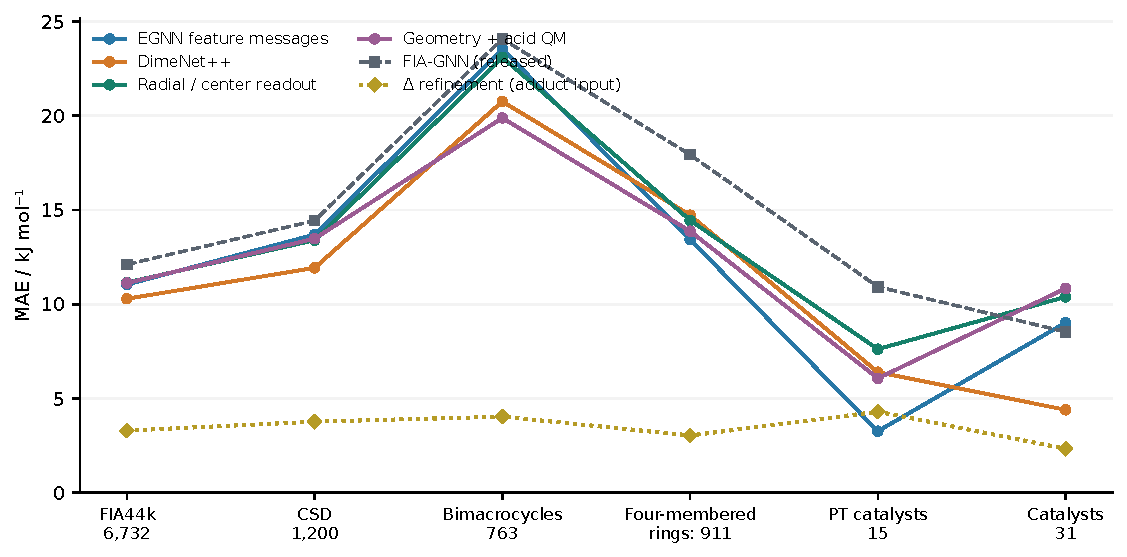
\includegraphics[width=.98\textwidth,height=.79\textheight,keepaspectratio]{figures/external_groups.pdf}
\caption{Ensemble MAE across all published test groups. The final row uses acid-plus-adduct quantum input; the other neural rows use optimized acid input.}
\end{figure}

\clearpage\section*{S13. Pnictogen-center comparison}
\begin{figure}[ht]\centering
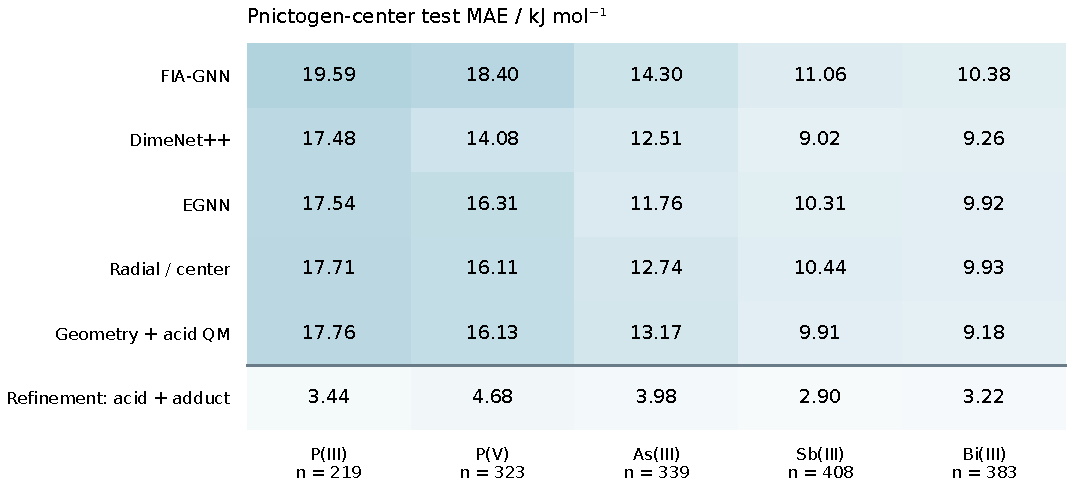
\includegraphics[width=.98\textwidth,height=.79\textheight,keepaspectratio]{figures/pnictogen_prediction.pdf}
\caption{Main-test class MAE for frozen ensembles and the quantum correction, with sample counts. Full 21-class exports accompany the code.}
\end{figure}

\clearpage\section*{S14. Molecular structure atlas}
\begin{figure}[ht]\centering
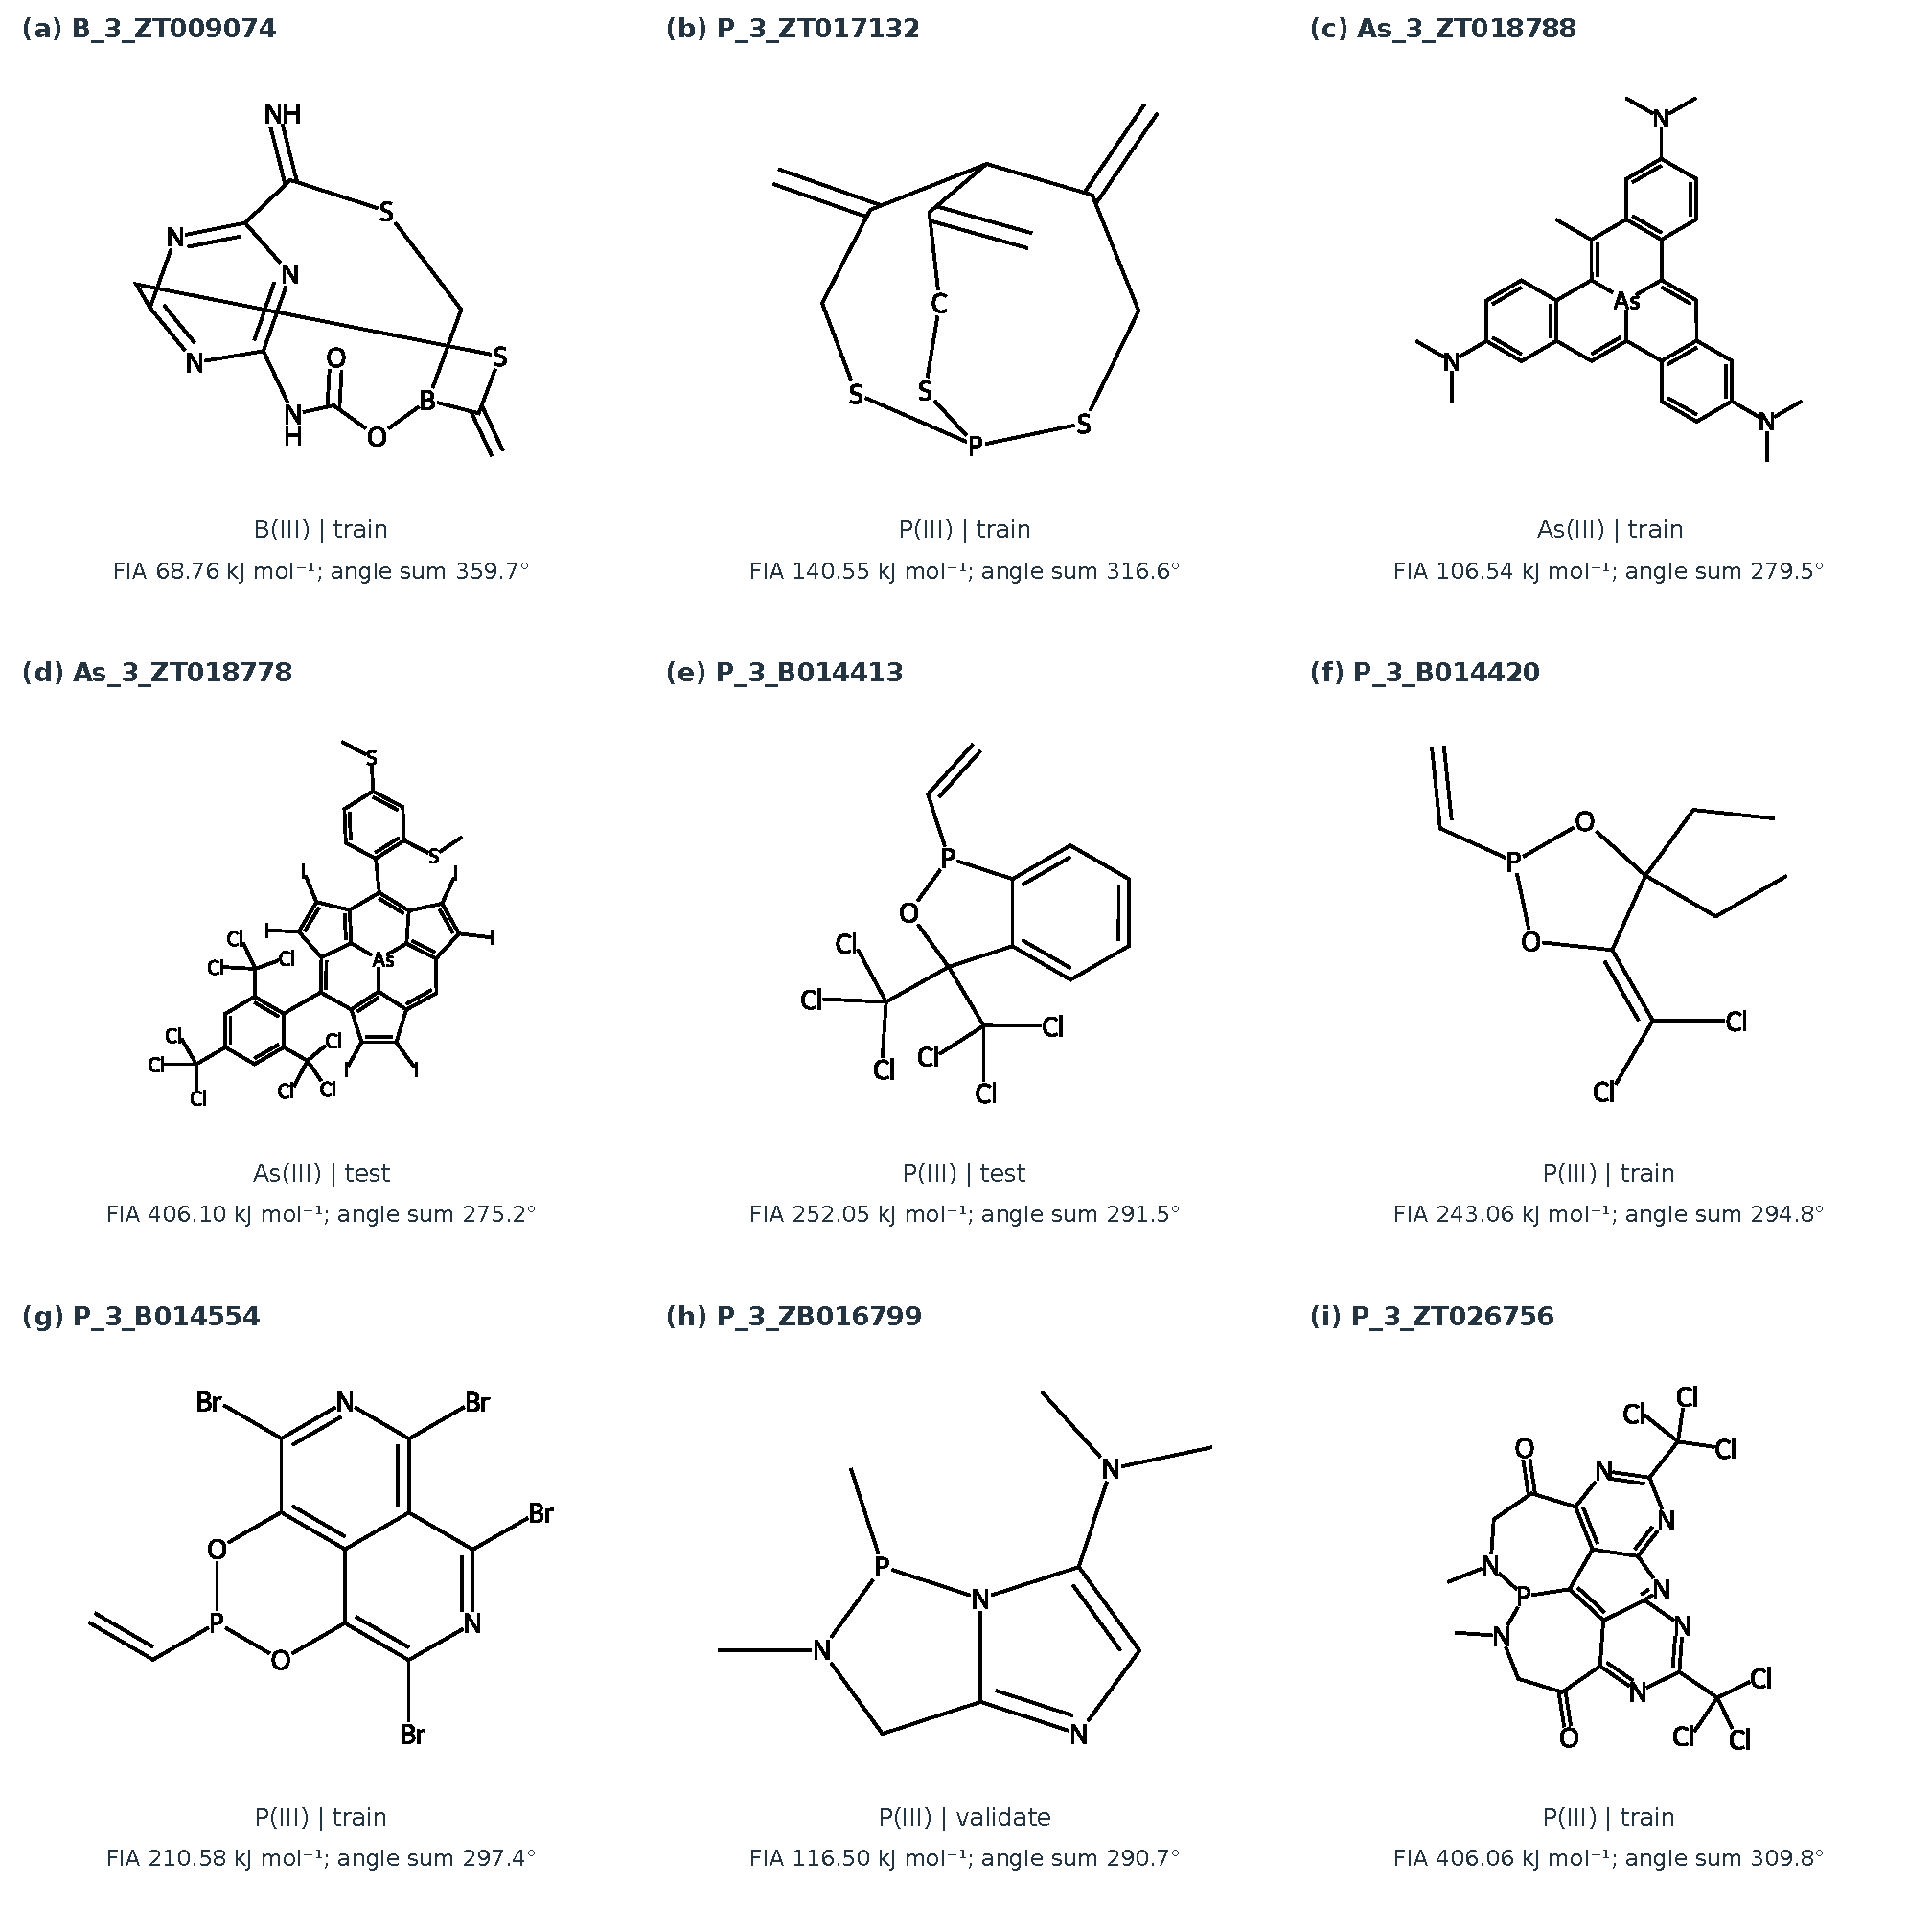
\includegraphics[width=.98\textwidth,height=.79\textheight,keepaspectratio]{figures/chemical_structure_atlas.pdf}
\caption{Nine chemically diverse FIA49k structures redrawn from released SMILES, with reference FIA, first-shell angle sum and partition membership. Training structures are illustrations; their fitted predictions are omitted.}
\end{figure}

\clearpage\section*{S15. Geometry-source overview}
\begin{figure}[ht]\centering
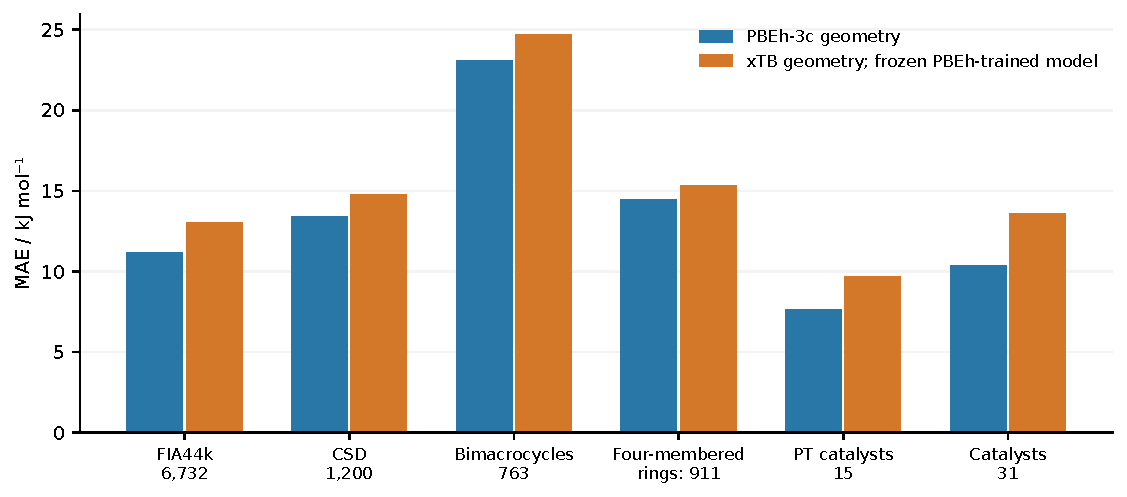
\includegraphics[width=.98\textwidth,height=.79\textheight,keepaspectratio]{figures/geometry_source_shift.pdf}
\caption{Frozen radial-ensemble errors for all six official test groups with PBEh-3c and GFN2-xTB acid coordinates.}
\end{figure}

\clearpage\bibliographystyle{unsrt}\bibliography{references}

\end{document}
